
% https://tex.stackexchange.com/questions/134773/label-variables-of-equation-using-tikz-without-using-itemize

\documentclass{article}

\usepackage{tikz}
\usetikzlibrary{matrix}
\usetikzlibrary{positioning}

\begin{document}

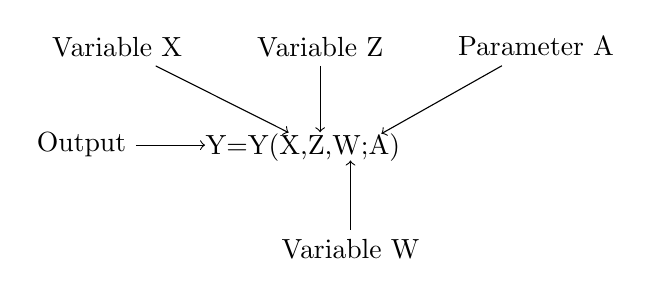
\begin{tikzpicture}

    \matrix[name=M1, matrix of nodes, inner sep=0pt, column sep=0pt]{
      \node (Y1) {Y}; & \node (equals) {=}; & \node (Y2) {Y}; & ( & \node (X) {X,}; & \node (Z) {Z,}; & \node (W) {W;}; & \node (A) {A}; & ) \\
    };

    \node (Output) [left=2.5em of Y1] {Output};
    \node (VariableZ) [above=2.5em of Z] {Variable Z};
    \node (VariableW) [below=2.5em of W] {Variable W};
    \node (VariableX) [left=2em of VariableZ] {Variable X};
    \node (ParameterA) [right=2em of VariableZ] {Parameter A};

    \draw[->] (Output) -- (Y1);
    \draw[->, shorten >=0.1em] (VariableZ) -- (Z);
    \draw[->, shorten >=0.2em] (VariableX) -- (X.north);
    \draw[->, shorten >=0.1em] (ParameterA) -- (A.north);
    \draw[->] (VariableW) -- (W);


\end{tikzpicture}

\end{document}
